\section{Transport between distant smoothed deletion measures}
\label{long:section}
\label{sec:long-palm}

The local comparison controls variations inside a mesoscopic cell.  We now
compare the smoothed deletion measures of two distant $R$-cells.  The
desired estimate is a squared $L^2$ distance $o(D^{-1})$ between their
square-root densities $s_v$ and $s_w$.  It follows from a common measure
whose likelihood is close to one in both augmented references.

The transport uses a route whose length may grow with $K$, so a fixed
density expense per step would be useless.  Instead we estimate the
second moment by comparing two transports with the same first tag.
When they change disjoint sets of labels, deleting the checks between
them separates their conditional integrals; the expense of restoring
these checks is determined by route encounters.  Random label choices
also make shared output coordinates rare.  Encounters
at the common first tag are unavoidable.  We keep an initial portion
unchanged in the observed copy and integrate out its partners in the
other copy.  Encounters confined to these silent portions then incur no
expense; encounters involving their seams are included in the count
$J_*$ of Proposition~\ref{rt:routes}.
The use of unnormalized conditional integrals extends the common-measure
comparison of \cite[Section~8]{H}; the sequential pinning and the estimates
that approach one are proved here.

Write $\mathcal A_{K,R}$ for the ordered pairs $(v,w)$ of $R$-cells whose
centres have forward first-coordinate displacement in $[.30K,.45K]$.
All averages over this set are normalized counting averages.  An error
$o_K(1)$ below tends to zero at fixed dilution along the thermodynamic
sequence, uniformly over the normalized nonnegative ground vectors under
consideration.  Constants may depend on the parameters fixed before $D$,
including $x$ and $j$, but never on $K$ or on a route length.

\begin{proposition}[Distant comparison of deletion measures]\label{long:comparison}
For sufficiently small $x>0$ relative to the previously fixed exponents,
the functions $s_v$ of Lemma~\ref{palm:reference} satisfy
\begin{equation}\label{long:hellinger}
 \frac1{|\mathcal A_{K,R}|}\sum_{(v,w)\in\mathcal A_{K,R}}
       \int |s_v(Y')-s_w(Y')|^2\,\dd Y'
       =o(D^{-1})+o_K(1).
\end{equation}
The $o(D^{-1})$ is uniform over the nonnegative ground vectors and over the
fixed window of $\alpha$.  The thermodynamic error is taken to zero first.
\end{proposition}

\subsection{The two-copy construction}

We retain the notation of Section~\ref{palm:section}: $\mathcal D$ is the
exposed data, $\mathcal I$ the unexposed labels, $B_i$ their plain bridge
laws, and $\lambda$ the conditional admissible bridge law.  For an $R$-cell
$v$, put $T_v=f_0D|v|$, $h_{v,i}=\1_{\{X_i\in v\}}$, and
$T_v^{\rm rel}=T_v^{-1}\sum_{i\ {\rm flagged}}h_{v,i}$.
The initial mass assigned to distinct tags $i,j$ is
\begin{equation}\label{long:tag-weight}
             \frac{h_{v,i}h_{w,j}}{T_vT_w}.
\end{equation}
Only tags in $\mathcal I$ and the retained data events of
Lemma~\ref{palm:omissions} will be used.  In particular the two cells have
bad-free neighborhoods of radius a sufficiently large constant times $R$.

To apply Proposition~\ref{rt:routes}, choose fixed lattice-cube
enlargements $Q_v,Q_w$ containing every candidate tag mean-site for the
respective cells.  Their sides are at most $C R$, and their $10R$ margins
lie in the retained bad-free neighborhoods.  Let $z$ be the first tag's
mean-site and put $Q=Q_w$.  The forward
displacements of the cell centres lie in $[.30K,.45K]$, so those from $z$
to all sites in $Q$ lie in $[.29K,.46K]$ when $K/R$ is sufficiently large.
Retain the route event $\mathcal E$ of that proposition as well as the
endpoint events already specified.  Conditional on the data and the two
mean-sites, sample its route using fresh randomness.  Its vertices are
distinct good sites.
At each interior site choose one available interior label uniformly,
excluding the tags.  Choices at different sites are independent.  If a
bounded number of additional exclusions is necessary, make it before the
uniform choice.  The supply estimate gives the bound
\begin{equation}\label{long:label-atom}
       \sup_l\Pr(\text{chosen label}=l\mid\mathcal D,
                         \text{route and tags})
                  \le \frac{C}{Df_0}.
\end{equation}
This gives a list of distinct labels
$i_0=i,i_1,\ldots,i_m=j$.  Consecutive bridge means have bounded distance.
The route is simple, so at most a fixed number of list entries have means
in any fixed-radius ball.  This bound does not depend on $m$.

Let $H_0=\lfloor R^{1/2}\rfloor$.  The silent prefix consists of the
vertices up to and including the last vertex within $H_0$ of the first
endpoint.  Define the silent suffix by reversing the route.  Proposition
\ref{rt:routes} shows that these pieces are disjoint and have length
$O(H_0)$.  Write their list indices as $0\le k<a_0$ and
$a_1<k\le m$.  Keep the prefix trajectories unchanged in the left copy
and the suffix trajectories unchanged in the right copy.  All trajectories
outside the list are unchanged in both copies.

The remaining paths are generated in the following order.
\begin{enumerate}
\item For $a_0\le k\le a_1+1$, generate a pair consisting of the left
path of $i_k$ and the right path of $i_{k-1}$.  Fix a unit cell at bounded
distance from both means as a measurable function of the exposed endpoints
alone, before sampling any latent or proposed paths.  Choose the common
midpoint uniformly in that cell, and use the two independent pinned bridge
laws given that midpoint.  Condition on
individual cutoffs, compatibility with every path retained in that copy,
and compatibility with earlier middle pairs.  Require also midpoint
$s$-separation from these opponents.  The probability of this event is at
least $1/2$, by Proposition~\ref{lp:insertion}; thus each step is a probability
kernel.  Fix any deterministic order for these middle steps.
\item For the remaining pairs, one member is already present as a retained
original.  If its midpoint $y$ is within $8b$ of the mean of the label to
be inserted and is $s$-separated from all paths already present in the
insertion copy, generate the other member with its pinned bridge law.
Impose all individual and compatibility checks, and divide this trial
measure by
\begin{equation}\label{long:pin-divisor}
                  \max\{1/2,p\},
\end{equation}
where $p$ is its total success probability.  If either preliminary midpoint
test fails, use the zero measure.  Use a fixed deterministic order within
each end.  Prefix pins occur in the right copy; suffix pins occur in the
left copy.  These kernels have mass at most one.
\end{enumerate}
Every generated path satisfies the constraints of its own copy.  The left
midpoint of $i_k$ is the right midpoint of $i_{k-1}$ for every $1\le k\le m$.
After deleting $i$ on the left and $j$ on the right the midpoint multisets
therefore coincide.  Order these baths with one common uniform permutation.
The weighted construction defines a finite common measure $\nu_{vw}$ on
the bath observation, with one lift to each augmented reference.

\begin{figure}[tbp]
 \centering
 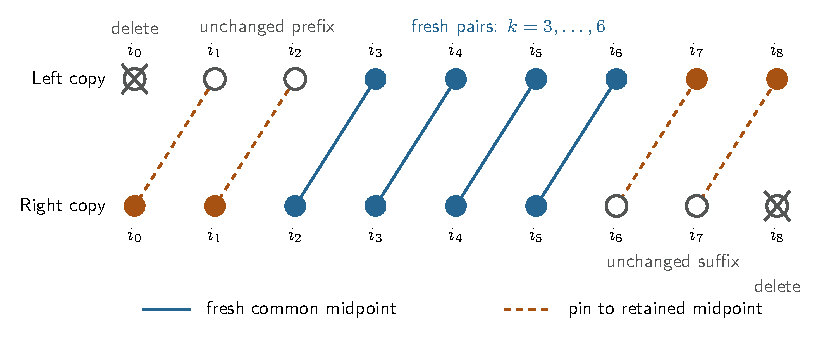
\includegraphics[width=\textwidth]{figures/transport.pdf}
 \caption{The midpoint pairing, shown schematically for $m=8$, $a_0=3$
 and $a_1=5$.  Each link identifies the left midpoint of $i_k$ with the
 right midpoint of $i_{k-1}$.  The middle pairs receive fresh common
 midpoints.  At each end one original trajectory is retained and its
 partner is pinned through the retained midpoint.  After deleting the
 crossed first left and last right tags, all remaining midpoints are
 paired.  The rows show label order, not geometric positions or paths.}
 \label{fig:transport}
\end{figure}

\begin{lemma}[Mass of the transport]\label{long:mass}
For some $c_3>0$, the mass of this common measure satisfies, after averaging
over $(v,w)\in\mathcal A_{K,R}$,
\begin{equation}\label{long:mass-bound}
 \nu_{vw}(1)\ge
       \E[T_v^{\rm rel}T_w^{\rm rel}]-C D^{-1-c_3}-o_K(1).
\end{equation}
\end{lemma}
\begin{proof}
The omitted tags, failed endpoint neighborhoods and route-existence
rejections have total weighted mass $O(D^{-1-c})+o_K(1)$ by
Lemma~\ref{palm:omissions} and Proposition~\ref{rt:routes}.  For the latter
use the marginal bad-site bound in an $O(R^3)$ neighborhood, the
exponentially small probability of a filled component reaching across the
margin, and the thermodynamically vanishing probability of a large
component.  Multiplying by the bounded number of relative-count factors
costs at most $D^{Cx}$, outside events smaller than any power of $D$.

It remains to check the subprobability steps near the two ends.  Use the
full-path count and motion event of Proposition~\ref{lp:good-probability} in the
enlarged endpoint neighborhoods solely to estimate the discarded mass;
it is not added to the conditional bridge law.  Its ordinary-original
motion tests give
$\sup_q|\omega(q)-Y|\le b$ and $\sup_q|\omega(q)-Z|\le b$ in the
chosen lift.  In particular its midpoint $y$ has distance at most $b$
from the source mean.  Consecutive means have distance bounded by a fixed
constant, which is at most $b$ after increasing the fixed cutoff constant.
Thus every required pin has $|y-m_{\rm insert}|\le2b<8b$.
The full-path event fails with weighted mass smaller than $D^{-1-c}$
after the $O(R^3)$ union bound.
On this event, a pinned trial with a separated midpoint has probability at
least $3/4$.  Indeed, start with the full original obstacle collection in
Proposition~\ref{lp:insertion}, delete any replaced originals, and add the
already generated paths.  Only boundedly many added paths can meet the
trial neighborhood, by simplicity of the route.  The last assertion of
that lemma applies to these additions.

For a middle path the necessary separation from a later pinned midpoint
was already checked in the copy containing the retained original that
provides that midpoint.  The paired middle paths have the same midpoint.
The two silent ends are separated by a distance of order $K$, so no check
joins them for sufficiently large $K$.  Thus the only remaining separation
failure is that a selected silent original has midpoint within $s$ of
another original midpoint.  In each bounded region the expected number
of such ordered pairs is at most $CD^2s^3$.  Summing the selected interior
labels uses \eqref{long:label-atom}; summing an end tag uses its factor
$T_v^{-1}$ or $T_w^{-1}$.  Enlarging all site sums to the endpoint
neighborhoods and using the other relative-count bounds gives at most
\[
 C R^3D^{Cx}\frac{D^2s^3}{Df_0}
       \le C D^{-7/5+3w+C'x}.
\]
The midpoint range failure is already covered by the displacement cutoffs
chosen above.  Outside these discarded events every pin has $p\ge3/4$,
so \eqref{long:pin-divisor} equals $p$ and the pin kernel has mass one.
Since $w$ and then $x$ were chosen small, all displayed losses have a
strict power saving beyond $D^{-1}$.  This proves the lemma.
\end{proof}

\subsection{Conditional likelihoods and the checks between two transports}

We next prove absolute continuity of the common measure's augmented lifts
and bound their second moments.  Denote the left lift density by
$\ell_{v,w}$.  Its reference has mass $\E T_v^{\rm rel}$, while its
own mass is $\nu_{vw}(1)$.  The mass estimate therefore shows why the
leading term sought for its second moment is
$\E[T_v^{\rm rel}(T_w^{\rm rel})^2]$: in the centered second moment
the three leading terms combine to
\[
 \E[T_v^{\rm rel}(T_w^{\rm rel})^2]
 -2\E[T_v^{\rm rel}T_w^{\rm rel}]+\E T_v^{\rm rel}
 =\E[T_v^{\rm rel}(T_w^{\rm rel}-1)^2].
\]
Lemma~\ref{palm:counts} controls this last expression.  The task below is
to bound the remaining second-moment error independently of route length.

For a fixed route and label
list let $S=\{i_k:k\ge a_0\}$ be the changed labels in the left copy.
The retained first tag $i$ is not in $S$.  Strip its factor $h_{v,i}/T_v$,
but keep the factor $h_{w,j}$ from the original second tag.  Denote the
resulting likelihood by $L_S$.  The division by $T_w$ and all choices
will be averaged at the end.

Here is an explicit integral defining $L_S$.  For fixed outside paths $o$
let $A_S(x;o)$ be the indicator of all reference checks incident to $S$,
including individual cutoffs, and let
\[
 Z_S(o)=\int A_S(x;o)\,\dd B_S(x),\qquad
 B_S=\bigotimes_{l\in S}B_l.
\]
Let $K_S(x,o;\dd z)$ be the subprobability kernel of the complete
two-copy construction, observed only in its changed left coordinates.
Its input $x$ consists of the latent original $S$ paths.  Define the
finite output measure
\begin{equation}\label{long:unnormalized-output}
 M_S(o;\dd z)=\int A_S(x;o)h_{w,j}(x)
                         K_S(x,o;\dd z)\,\dd B_S(x).
\end{equation}
On reference-admissible configurations,
\begin{equation}\label{long:exact-likelihood}
                         L_S(z,o)=\frac{\dd M_S(o)}{\dd B_S}(z).
\end{equation}
To verify this, both the conditional input law and the conditional reference
output law have the same divisor $Z_S(o)$.  It cancels in their likelihood
ratio, as in Lemma~\ref{palm:likelihood}.  Absolute continuity follows from
the ordinary densities of middle outputs and the distinct latent midpoint
sources for pinned left outputs.  A detailed density bound is proved below.

For upper bounds, integrate out all right pins against the silent prefix.
They occur after the middle steps and are subprobability kernels.  The
left suffix pins do not use these right paths.  Removing these right kernels
therefore increases \eqref{long:unnormalized-output}.  In the rest of the
upper-bound argument $K_S$ denotes this enlarged kernel.  This operation
is the reason that meetings confined to two silent prefixes cost nothing.

Fix two route and label choices with the same first tag, with changed sets
$S,T$ and second tags $j,j'$.  Fix the paths outside $U=S\cup T$, at a value
where the regular conditional reference law is defined.  Every statement
until the averaging subsection is uniform in these fixed allowed values.
Let $Z_U$ be the reference normalizer on $U$ relative to $B_U$.

Define the separate $S$ protocol by deleting the old paths indexed by
$T\setminus S$ from its outside obstacles and removing each check against
such a path.  Keep its list of generated transitions unchanged.  In
particular a right middle path keeps the endpoints of its label even when
that label's old trajectory has been deleted as a left obstacle.  Define
the separate $T$ protocol symmetrically.  Use a superscript minus for these
protocols and write $A_S^-,Z_S^-,M_S^-$ for their reference indicator,
reference normalizer and unnormalized output measure.

These separate quantities depend on their own latent and output variables
and on the common fixed outside of $U$.  They do not depend on the other
set's unshared path variables.  The only apparent exception is the first
right middle insertion at the edge of a silent prefix.  Its old trajectory
is retained on the left, but its right insertion uses only the fixed
endpoints; all checks using the old trajectory are among the deleted
outside checks.  The right pins have already been integrated out.
This verifies the asserted independence also at that edge.

We now specify exactly which comparisons can contribute a cost.  Each
reference check between a label of $S\setminus T$ and a label of
$T\setminus S$ is an edge of a finite graph on these two sets.  Each
deleted proposal check gives a second kind of edge: one end records its
generated transition and the other the removed old opponent label.  A
transition has at most two generated paths, one in each copy.  A label
appears as a primary path once and as an auxiliary path at most once.
The fixed confinement radii imply that a check is identically satisfied
unless the associated route sites have distance at most a fixed $r_c$.
For a predecessor or a midpoint source use the neighboring route site.
Increase $r_c$ once to include these bounded displacements.

Let $J$ be the full site-contact count of Proposition~\ref{rt:routes}, and
$J_*$ its contact count between the changed portions from the common end,
with these step neighbors included.  There are at most $CJ_*$ edges in the
graphs just defined, hence at most $CJ$ edges.  Every degree is bounded by
a constant: a simple lattice route contains only boundedly many vertices
in an $r_c$-ball.  The constants in this assertion do not count the route
length.

For a check between distinct labels $l,k$ put
\begin{equation}\label{long:beta}
 \beta_{lk}=b_D\left(1+\frac1{s\vee d(Y_l,Y_k)}
                       +\frac1{s\vee d(Z_l,Z_k)}\right),
 \qquad b_D=\frac{C(\log D)^C}{D}.
\end{equation}
For a pinned trial with midpoint $y$ checked against an old path $X_k$, also
put
\begin{equation}\label{long:midpoint-cost}
                 m(y,X_k)=\frac{b_D}{s\vee d(y,X_k(0))}.
\end{equation}
All compared labels are distinct, even when the sets $S,T$ intersect:
an outside obstacle is never the label currently inserted.  Lemma
\ref{lp:collision} bounds each corresponding collision or uniform-midpoint
separation cost by $C\beta_{lk}$, and a pinned collision by
$C(\beta_{lk}+m(y,X_k))$ when the pin satisfies separation.  Since
$s=D^{-4/5}$, all these costs are at most $CD^{-19/100}$ for large $D$.
Let $B_{ST}$ be the sum of the $\beta$ costs over all affected checks,
with their bounded multiplicities, and let $M_{ST}$ be the corresponding
sum of \eqref{long:midpoint-cost}.  Thus
\begin{equation}\label{long:worst-cost}
      B_{ST}+M_{ST}\le C D^{-19/100}J.
\end{equation}

\subsection{Reference normalizers and proposal probabilities}

There are two different sources of cost in the product of likelihoods.
Checks between distinct labels prevent the two conditional integrals from
factoring; the next two lemmas compare the reference normalizers and the
proposal probabilities when these checks are removed.  If a label belongs
to both changed sets, its output coordinate is also shared by the two
likelihoods.  We will treat those coordinates separately, by bounding
selected output marginals.

The normalization calculation uses one-path insertion bounds even when
the number of changed paths is large.  No joint normalizer is bounded
below by a constant independent of that number.

\begin{lemma}[Reference normalizers]\label{long:normalizers}
If $S\cap T=\varnothing$, then
\begin{equation}\label{long:disjoint-normalizers}
       1\le\frac{Z_S^-Z_T^-}{Z_U}
                    \le \exp(CB_{ST}).
\end{equation}
If $q=|S\cap T|$ is arbitrary, then
\begin{equation}\label{long:shared-normalizers}
       \frac{Z_S^-Z_T^-}{Z_U}
                    \le C^q\exp(CB_{ST}).
\end{equation}
All normalizers are strictly positive.  In the disjoint case, if $H$ is
any measurable function of the latent originals with $0\le H\le1$, and
$A^- = A_S^- A_T^-$, then
\begin{equation}\label{long:tag-integral-difference}
 0\le \frac1{Z_U}\int H(A^- - A_U)\,\dd B_U
                       \le C e^{CB_{ST}} B_{ST}.
\end{equation}
\end{lemma}
\begin{proof}
The conditional distribution of any one original path, given all the
others, is bounded by $c_0^{-1}B_l$ with $c_0=3/4$, by
Proposition~\ref{lp:insertion}.  This remains true after arbitrary checks have
been removed.  Every reduced normalizer is positive by inserting its
coordinates successively; the resulting lower bound may depend on their
number and is used only for positivity.

Suppose first that $S,T$ are disjoint.  With their cross checks removed the
integral factorizes as $Z_S^-Z_T^-$.  Add the cross checks in any fixed
order.  For a check between $l$ and $k$, condition on all paths except
$l$.  Its failure probability is at most $c_0^{-1}\beta_{lk}$.
Consequently this insertion multiplies the inverse normalizer by at most
\[
 (1-c_0^{-1}\beta_{lk})^{-1}
                         \le \exp(2c_0^{-1}\beta_{lk})
\]
for large $D$.  Multiplication gives
\eqref{long:disjoint-normalizers}.  Under the normalized product with all
cross checks deleted, their union fails with probability at most
$c_0^{-1}\sum\beta_{lk}$.  Dropping $H\le1$ and using the normalizer
ratio proves \eqref{long:tag-integral-difference}.

For general $S,T$, put $A=S\cap T$.  Delete the labels of $A$ and their
incident checks from both separate reference integrals.  This increases
$Z_S^-$ and $Z_T^-$.  The remaining sets $S\setminus A,T\setminus A$
are disjoint, so the preceding comparison applies to them.  Their joint
normalizer is at most $c_0^{-q}Z_U$, since one can add the $q$ labels in
$A$ using their uniform insertion lower bounds.  The cross-check costs
used for the disjoint remainder are among those in $B_{ST}$.  These two
inequalities prove \eqref{long:shared-normalizers}.
\end{proof}

\begin{lemma}[Comparison of transition factors]\label{long:transitions}
Use the same latent originals and the same generated variables in the
original and separate protocols.  The original integrand is bounded by
the separate integrand times a nonnegative factor $\mathcal R$ satisfying
\begin{align}
 \mathcal R&\le e^{C D^{-19/100}J},
                                  \label{long:factor-exponential}\\
 \mathcal R&\le 1+C e^{C D^{-19/100}J}(B_{ST}+M_{ST}).
                                  \label{long:factor-increment}
\end{align}
The assertion is for the product of the two protocols as well.  A
transition with no removed check has ratio exactly one.
\end{lemma}
\begin{proof}
Fix the history before one generated pair or pin.  Its proposal law
before checks is unchanged by deletion of outside obstacles.  Let $p$
and $p^-$ be the acceptance probabilities with and without the removed
checks; then $p\le p^-$.  For a middle pair $p\ge1/2$, and hence
\[
             \frac{p^-}{p}\le 1+2(p^- -p).
\]
For a pin, use $w=\max(1/2,p)$ and $w^- =\max(1/2,p^-)$.  The map
$p\mapsto\max(1/2,p)$ is increasing and $1$-Lipschitz, so
\[
             \frac{w^-}{w}\le 1+2(p^- -p).
\]
The ratio of admissibility indicators is bounded by one in this upper
comparison.  A midpoint separation indicator outside the pin proposal
can also be increased.  On the support of the old nonzero integrand, its
midpoint is separated from every old opponent, so the pinned collision
estimate applies.  Off that support the inequality is automatic.  The
capped expression \eqref{long:midpoint-cost} thus gives a valid bound
everywhere.

For a middle proposal the union bound gives
$p^- -p\le C\sum\beta_{lk}$ over its removed checks.  For a pin the
bound is $C\sum(\beta_{lk}+m(y,X_k))$.  The proposal may be a coupled
pair, but the removed checks involve one of its two marginals, and the
uniform-midpoint insertion bounds apply to those marginals.  Conditioning
the original proposal does not enter this estimate of $p^- -p$.

Multiplying the displayed ratio bounds over the affected transitions of
both protocols gives
$\mathcal R\le\exp(C(B_{ST}+M_{ST}))$.
The inequalities $e^a-1\le ae^a$ and
\eqref{long:worst-cost} give both conclusions.  Unaffected transitions
have identical numerators and divisors at the same history.  Thus the
number of factors actually paid is bounded by the number of graph edges,
not by the number of generated transitions.
\end{proof}

\subsection{Marginals of selected output paths}

Before multiplying likelihoods with shared labels, we record the precise
form of reverse integration used for their common output coordinates.
Only primary marginals of a coupled pair are bounded.  Its full two-copy
law has equal midpoints and is not dominated by a product of free bridges.

\begin{lemma}[Selected outputs of sequential kernels]\label{long:kernel}
Let $\mu(\dd x)$ be a probability measure of latent variables, followed by
a finite ordered list of subprobability kernels.  At stage $r$ the kernel
generates a primary variable $z_r$ and arbitrary auxiliary variables.  Let
$Q$ be a set of stages.  Suppose that, for every latent input and every
allowed preceding history, the primary marginal at $r\in Q$ is at most
$A_r\nu_r(x,\dd z_r)$, where $\nu_r$ is a subprobability kernel depending
on $x$ but not on the preceding history.  Then the joint measure of the
selected primary outputs is at most
\begin{equation}\label{long:reverse-kernel}
       \left(\prod_{r\in Q}A_r\right)
                   \int\mu(\dd x)\prod_{r\in Q}\nu_r(x,\dd z_r).
\end{equation}
\end{lemma}
\begin{proof}
Integrate an arbitrary nonnegative measurable test function of the selected
outputs.  Starting with the last stage, integrate every unselected stage
using its mass bound one.  At a selected stage integrate its auxiliary
variables and use the primary marginal bound.  The new test function
depends on the latent input and the earlier selected outputs, but no
longer on the history variables generated at this stage.  Induction
backwards through the finite list proves \eqref{long:reverse-kernel}.
The argument first applies to bounded tests and then to all nonnegative
tests by monotone convergence.
\end{proof}

\begin{lemma}[Uniform marginal bound]\label{long:shared-density}
Divide the separate output measure $M_S^-$ by its reference normalizer
$Z_S^-$, and omit its original tag indicator if desired.  For any $q$
specified primary output labels, its marginal is dominated by
\begin{equation}\label{long:marginal-bound}
                 G_D^q\bigotimes_{l\text{ specified}} B_l,
              \qquad G_D=C D^{C\sqrt x}.
\end{equation}
The same assertion holds for $T$, and the constants are independent of
the number of unselected outputs.
\end{lemma}
\begin{proof}
The normalized separate latent-original law is its admissible product
bridge law.  A middle stage, conditional on all these originals and on
the preceding history, has primary marginal at most
$C D^{Cx}B_l$, by Corollary~\ref{lp:trial-density} and its acceptance
probability at least $1/2$.  A pin has primary conditional bridge law at
most $2\1_{\rm range}(y) B_l(\dd z\mid z(0)=y)$, where $y$ is the
midpoint of its retained original partner and
$\1_{\rm range}(y)=\1_{\{|y-m_l|\le8b\}}$; all separation and avoidance
indicators are discarded in this upper bound, so the retained cutoff is
independent of the preceding history.  This cutoff conditional bridge is
the kernel $\nu_r$ in Lemma~\ref{long:kernel}.  Both estimates hold
uniformly in the history, including
histories obtained after deleting some outside checks.

Apply Lemma~\ref{long:kernel} to the specified stages.  For each specified
pin its source is a latent original in $S$: these sources lie in the
right-silent suffix.  The sources for distinct pins are distinct labels.
If there are $p$ specified pins, their joint latent-source marginal is
bounded by $C^p$ times the corresponding product bridge law, by
Corollary~\ref{lp:trial-density}.  Indeed the uniform conditional one-path
density bound survives integration over any other latent coordinates and
can then be iterated over these $p$ coordinates.

Let $a(l)$ be the source label of the pin with output label $l$.  Integrating
out all parts of its source other than the midpoint gives
$g_{a(l)}(y)\,\dd y$.  On the retained range, neighboring means and
the Gaussian ratio bound~\eqref{lp:midpoint-ratio} give
$g_{a(l)}(y)\le C D^{C\sqrt x}g_l(y)$.  Therefore
\[
 \int \1_{\rm range}(y)g_{a(l)}(y)
           B_l(\dd z\mid z(0)=y)\,\dd y
                         \le C D^{C\sqrt x}B_l(\dd z).
\]
Use this for each distinct source.  Together with the middle-output
bounds it proves \eqref{long:marginal-bound}.  No assertion of independence
between a pin and its source midpoint has been used: the midpoint is
integrated against the conditional bridge before the resulting free
bridge bound is obtained.
\end{proof}

\subsection{The product of two likelihoods}

\begin{lemma}[Disjoint and shared changed sets]\label{long:product}
At almost every fixed admissible outside of $U=S\cup T$, the likelihoods
of the two original transports satisfy the following bounds.  If $S,T$
are disjoint, then
\begin{equation}\label{long:disjoint-product}
 \E[L_SL_T\mid U^c]\le
 \E[h_{w,j}h_{w,j'}\mid U^c]
 +C e^{C D^{-19/100}J}
          \bigl(B_{ST}+J_*b_D(1+t^{-3/2})\bigr).
\end{equation}
If $q=|S\cap T|\ge1$, then
\begin{equation}\label{long:shared-product}
          \E[L_SL_T\mid U^c]
                     \le e^{C D^{-19/100}J}G_D^q,
\end{equation}
after increasing the fixed constant in $G_D$.
\end{lemma}
\begin{proof}
By \eqref{long:exact-likelihood} and the enlargement of the kernels, the
conditional product integral is bounded by the integral using
the free output measure $B_U$, the union admissibility indicator, and the
single divisor $Z_U$.  In each likelihood keep a separate set of latent
original variables.  These copies are not identified even if $S,T$ have
common labels.  Only shared output coordinates are identified by the
integration against $B_U$.

Suppose first that the sets are disjoint.  Apply Lemma
\ref{long:transitions}, delete the union output-admissibility indicator in
an upper bound, and integrate with the separate protocols.  The term one
in \eqref{long:factor-increment} has integral at most
\[
 \frac1{Z_U}
       \int A_S^-(x)A_T^-(x')h_{w,j}(x)h_{w,j'}(x')
                              \,\dd B_S(x)\dd B_T(x').
\]
Here the generated kernels were integrated using their mass bounds one.
By \eqref{long:tag-integral-difference} this is at most the reference
expectation of $h_{w,j}h_{w,j'}$, plus
$Ce^{CB_{ST}}B_{ST}$.  The terms from $B_{ST}$ in
\eqref{long:factor-increment} are bounded by the same normalizer ratio
and the masses of the separate normalized protocols, each at most one.

Consider one term $m(y,X_k)$ of $M_{ST}$.  Its midpoint $y$ belongs to
a latent original of one separate protocol, whereas $X_k$ is an output
path of the other.  Conditional on the fixed outside the two extended
protocol measures are independent.  On the side providing $y$, drop its
tag indicator and integrate all generated transitions.  The marginal of
the source original is bounded by a fixed constant times its free bridge.
For every fixed point $z$, the Gaussian midpoint density then gives
\begin{align*}
 \int_{d(y,z)\le C_b}\frac{g_l(y)}{s\vee d(y,z)}\,\dd y
 &\le \|g_l\|_\infty\int_{|u|\le1}|u|^{-1}\,\dd u
            +\int_{d(y,z)>1}g_l(y)\,\dd y\\
 &\le C(1+t^{-3/2}).
\end{align*}
The local range $C_b$ suffices because all other checks vanish; nearby
lifts or the periodized Gaussian give the same estimate.  This calculation
does not require a density bound for the opposing output midpoint.
There are at most $CJ_*$ such terms.  Use
\eqref{long:disjoint-normalizers} for the normalizer ratio and absorb its
exponent using \eqref{long:worst-cost}.  This proves
\eqref{long:disjoint-product}.

For intersecting sets use \eqref{long:factor-exponential}.  After dropping
union admissibility, write the separate output measures as $Z_S^-f_S B_S$
and $Z_T^-f_T B_T$, with the original tag indicators included.  Integrating
unshared output coordinates leaves the product of their marginals on
$A=S\cap T$.  By Lemma~\ref{long:shared-density}, one of these marginal
densities is at most $G_D^q$; the other has integral at most one.  Thus the
free output integral is at most $Z_S^-Z_T^-G_D^q$.  Division by $Z_U$,
\eqref{long:shared-normalizers}, and absorption of $C^q$ in $G_D^q$
prove \eqref{long:shared-product}.
\end{proof}

\subsection{Averaging labels, routes and endpoints}

We now return to the original augmented reference and its left lift
density $\ell_{v,w}$.  It is zero on omitted first tags or rejected data.
On retained data and
first tag $i$ it is the sum of $L_S/T_w$ over the candidate second tags,
averaged over the route and interior-label choices.  Squaring this sum
produces exactly two independent choices with common first tag $i$ and
the same underlying data.  In particular the data are never independently
resampled when the likelihood is squared.

\begin{lemma}[Endpoint sums and label matches]\label{long:label-average}
At fixed retained data and route sites, the label average of the error in
\eqref{long:disjoint-product}, together with the contribution of all
choices having $S\cap T\ne\varnothing$, is at most
\begin{equation}\label{long:label-error}
                C D^{-1+\zeta(x)}J_*e^{\delta_D J},
             \qquad \delta_D\longrightarrow0,
             \qquad \zeta(x)\longrightarrow0\quad(x\downarrow0).
\end{equation}
This estimate includes the normalized sums over the three tag labels at
their specified mean-sites.  The remaining weight of each tag site is
at most $CR^{-3}$.
\end{lemma}
\begin{proof}
Every possible mean-site of an end tag lies in the corresponding $R$-cell
enlarged by a fixed radius.  At each site the number of eligible tags is
at most $Cf_0D$, by the endpoint count estimate.  Since
$T_v=T_w=f_0DR^3$, their counting sums with $h\le1$ are dominated by a
site weight $CR^{-3}$ and a label subprobability measure with maximum atom
$C/(Df_0)$.  These are deterministic upper bounds at the fixed data;
the site weights will be removed before any environmental expectation.
Zero or very small tag families cause no problem: their extracted label
measure simply has mass less than one.  Interior selections are probability
measures and have the same maximum-atom bound
\eqref{long:label-atom}.

For any fixed endpoint $z$, a dyadic decomposition of the endpoint count
bound in Definition~\ref{lp:certificate} gives, for a candidate label family
in a bounded neighborhood,
\begin{equation}\label{long:endpoint-average}
 \frac{C}{Df_0}\sum_l\frac1{s\vee d(z,Y_l)}
          \le C\left(1+\frac{D^{1/100}}{Df_0s}\right)\le C,
\end{equation}
and the same holds for the $Z$ endpoints.  To see the first inequality,
sum separately the innermost ball of radius $s$ and the shells
$2^as<d\le2^{a+1}s\le C_b$.  The volume term sums as a geometric
series of order $Df_0$, whereas the additive $D^{1/100}$ term sums to
$CD^{1/100}/s$.  Here $D^{1/100}/(Df_0s)=D^{-19/100+x}$ is bounded
for small $x$.

Every edge contributing a $\beta$ cost has a label choice on at least one
side which is free to average: the common first tag is outside both changed
sets.  For an interior label use \eqref{long:endpoint-average} conditional
on the tags; for an end-tag label use the same bound in its candidate
family at its fixed mean-site.  Coincidence exclusions may be removed in
this positive upper bound, because the reciprocal distance is capped at
$s$.  Thus each averaged $\beta$ costs at most $Cb_D$, and there are at
most $CJ_*$ edges.  The midpoint cost in
\eqref{long:disjoint-product} has already been integrated.  This bounds
the disjoint error by
\[
       C e^{C D^{-19/100}J}J_*b_D(1+t^{-3/2}).
\]

For the intersecting choices let $\mathcal E$ be all pairs of slots in
the two changed lists whose label choices could agree.  Its cardinality
is at most $CJ_*$, with all such pairs among the $CJ$ full contacts.
Because each list has distinct labels, the actual matches form a matching:
no slot belongs to two of them.  The product label measure assigns each
prescribed set of $h$ disjoint matches mass at most $(C/(Df_0))^h$.
For interior matches,
this follows by conditioning on the tags and then on one list, and using
independence between sites in the other list.  A tag can match an interior
slot only at its one possible base site.  For a match of the two second
tags, sum one tag with the same maximum-atom bound.  There are only two
noncommon tag slots, so their exclusions change these bounds by a fixed
factor per prescribed match, independent of the route length.

The tag measures have mass at most one, so summing the remaining tag
variables cannot increase this bound.

Expand
\[
 G_D^q=\prod_{e\in\mathcal E}
             \bigl(1+(G_D-1)\1_{\{e\ {\rm matched}\}}\bigr).
\]
To restrict to at least one match, designate one matched edge and bound
the remaining product in the same way.  The preceding probability bound
and the elementary inequality $(1+a)^M\le e^{aM}$ give
\begin{equation}\label{long:match-sum}
 \E_{\rm labels}[\1_{\{q>0\}}G_D^q]
       \le \frac{C G_D}{Df_0}J_*
                         \exp\left(\frac{C G_D}{Df_0}J\right).
\end{equation}
Use this in \eqref{long:shared-product}.  Since
$G_D/(Df_0)=C D^{-1+x+C\sqrt x}$, the coefficient in this last
exponent tends to zero.  Absorb the fixed powers of $\log D$ in an
arbitrarily small power depending on $x$, and combine the two estimates.
They have the form \eqref{long:label-error}, with for example
$\delta_D=C D^{-19/100}+C G_D/(Df_0)$.  This proves the lemma.
\end{proof}

The next step is the only place where the environment is averaged in the
likelihood estimate.  The two routes share that environment.  For each
deterministic common endpoint, Proposition~\ref{rt:routes} supplies
\[
 \E[\1_{\rm retained}e^{\kappa J}]\le C,
 \qquad
 \E_{\rm sites}\E[\1_{\rm retained}\1_{\{J_*>0\}}]
                                                \le CR^{-c_g}.
\]
The second average is over the two independent noncommon sites with
weights at most $CR^{-3}$ each.  The deterministic bounds in
Lemma~\ref{long:label-average} allow precisely this site average even
though the actual candidate tag counts depend on the environment.
For large $D$, $J^2e^{2\delta_DJ}\le C_\kappa e^{\kappa J}$.
As $J_*\le J$, Cauchy--Schwarz consequently gives
\begin{equation}\label{long:route-average}
 \E_{\rm sites}\E[
     \1_{\rm retained}J_*e^{\delta_DJ}]
                      \le C R^{-c_g/2}.
\end{equation}
Uniformity in the common endpoint permits its remaining average as well.
Combining \eqref{long:label-error} and \eqref{long:route-average} bounds
the averaged likelihood error by
$C D^{-1+\zeta(x)-wc_g/2}$.  Choose $x$ small enough that
$\zeta(x)<wc_g/4$.  This has a strict power saving beyond $D^{-1}$.

\begin{proposition}[Augmented moments]\label{long:augmented-moments}
For some $c_4>0$, the left augmented likelihood satisfies
\begin{equation}\label{long:second-moment}
 \int\ell_{v,w}^2\,\dd P_{{\rm aug},v}
       \le \E[T_v^{\rm rel}(T_w^{\rm rel})^2]
                           +CD^{-1-c_4}+o_K(1)
\end{equation}
after averaging over $\mathcal A_{K,R}$.  Its mass satisfies
\eqref{long:mass-bound}, and the same estimates hold with $v,w$ exchanged.
\end{proposition}
\begin{proof}
In the expansion of the squared likelihood keep the common first-tag
factor $h_{v,i}/T_v$.  Conditional on the outside of $S\cup T$ it is
fixed, because neither changed set contains $i$.  Apply
Lemma~\ref{long:product} to the two choices.  The conditional expectation
in its disjoint leading term is exactly the original expectation of the
two end-tag indicators.  All tag choices, route choices, and interior
label choices are fixed independently of the latent paths, conditional
on the data.  We may therefore sum this leading term on the original
path space.  Removing all good-event and noncoincidence restrictions in
this nonnegative upper bound yields
\[
 \E\left[
    \left(\sum_i\frac{h_{v,i}}{T_v}\right)
    \left(\sum_j\frac{h_{w,j}}{T_w}\right)^2\right]
             =\E[T_v^{\rm rel}(T_w^{\rm rel})^2].
\]
The errors and intersecting choices are controlled by
Lemma~\ref{long:label-average} and \eqref{long:route-average}.  This
proves \eqref{long:second-moment}.  The mass bound is
Lemma~\ref{long:mass}.  For the right augmented estimate keep the same
two-copy construction, and hence the same common measure.  Reverse only
the list indexing and designate the right copy primary; retain the actual
chronological order of the generated middle kernels.  Its common endpoint
is then the last tag and its silent prefix is the previous silent suffix.
The kernels pinned into the left copy can now be integrated out.  The
remaining right pins do not use them: the two end families lie in opposite
copies, and no check joins the separated endpoint neighborhoods.  Every
kernel estimate and the reverse-integration lemma hold for an arbitrary
fixed middle order, so this change of designation requires no resampling
or reversal of the sampling order.

The original retention also gives the event required for the reversed
route comparison.  The fixed endpoint cube $Q_v$ and its $10R$ margin
are bad-free.  For every filled bad component, the actual first endpoint
lies outside its fill by the original route event.  Since $Q_v$ is
nearest-neighbor connected and contains that endpoint, a path in $Q_v$
cannot enter the fill without meeting the bad component.  Thus every site
of $Q_v$ lies outside every such fill.  The component-size cutoff is
unchanged, so Proposition~\ref{rt:routes} applies with the common terminal
endpoint and the noncommon endpoints in $Q_v$.
The preceding calculation therefore gives the right augmented estimates
for the original common measure.
\end{proof}

\begin{proof}[Proof of Proposition~\ref{long:comparison}]
The augmented reference has mass $\E T_v^{\rm rel}$, while its common
measure has mass $\int\ell_{v,w}\,\dd P_{{\rm aug},v}$.  Subtract twice
the mass lower bound from the second-moment upper bound and add the
reference mass.  Proposition~\ref{long:augmented-moments} gives
\begin{equation}\label{long:centered-second}
 \int|\ell_{v,w}-1|^2\,\dd P_{{\rm aug},v}
 \le \E[T_v^{\rm rel}(T_w^{\rm rel}-1)^2]
                                      +o(D^{-1})+o_K(1)
\end{equation}
in the normalized pair average.  The likelihood remains zero on the
omitted reference events; their loss was included in the mass estimate.

Outside the negligible count tails, $T_v^{\rm rel}\le C/f_0$.
Lemma~\ref{palm:counts} and the uniform marginal weights of the ordered
cell pairs therefore bound the main term of
\eqref{long:centered-second} by
\[
 C D^x\bigl(D^{-1-w/6}+D^{-1+x}R^{-3}\bigr)
     \le C\bigl(D^{-1-w/6+x}+D^{-1+2x-3w}\bigr)
                                      =o(D^{-1}).
\]
The removed count tails remain negligible after multiplication by the
relative counts, by the bookkeeping in Lemma~\ref{palm:counts}.  Choose
$x<w/12$, in addition to its preceding restrictions.  The same centered
bound holds in the right augmented reference.

For finite measures $P$ and $\nu\ll P$ with likelihood $\ell$, their
squared Hellinger distance is
$\int(1-\sqrt\ell)^2\,\dd P\le\int(1-\ell)^2\,\dd P$.
Projection cannot increase this distance: conditional Cauchy--Schwarz
increases the affinity and preserves both masses.  Project both augmented
comparisons to the common ordered bath.  Their reference densities are
$s_v^2$ and $s_w^2$, by Lemma~\ref{palm:reference}, and their
common projected density is that of $\nu_{vw}$.  The triangle inequality
in $L^2$ and the two bounds \eqref{long:centered-second} now imply
\eqref{long:hellinger}.  Every volume-dependent rejection was recorded
as $o_K(1)$ at fixed dilution; taking that limit before $D\to\infty$
completes the assertion.
\end{proof}
